\section{Introduction}

This chapter introduces the three open innovation cases recruited for this study. We begin with an overview of each case before comparing them in terms of the number of participants, their demographic and psychological attributes, spatial proximity to one another, knowledge sharing ties, and broker roles. All three cases are quite different, and by the end of this chapter, the reader ought to have a good understanding of each. Without this understanding, it will be harder for the reader to make sense of the results from the exponential random graph modelling and analysis of semi-structured interviews presented in the chapters that follow.

\section{Case overviews}

The distinguishing features of each case are listed in Table \ref{tab:cases}. We are dealing with a small number of individual participants in each case. It is important to note that two of the cases were at an early stage of execution (i.e. they were relatively new partnerships), while the third was in its closing stage at the time of data collection (the partnership was well-established and had achieved its primary goal). Case 1 is an example of inbound open innovation, Case 2 is about coupled open innovation, whereas Case 3 is a mixture of outbound and coupled open innovation \citep{gassmann2004towards}. One can characterise innovation as either incremental or radical \citep{ettlie1984organization}. Incremental innovation is about improvements within an existing framework (becoming better at what we already do) whereas radical innovation is a change of frame (doing something we did not do before) \citep{norman2014incremental}. Case 1 is mostly about incremental innovation whereas Case 2 and 3 are more about radical innovation.

\begin{sidewaystable}[hbt!]
\centering
\resizebox{0.9\textwidth}{!}{%	
\begin{threeparttable}
\footnotesize
\setlength{\tabcolsep}{6pt}
\renewcommand{\arraystretch}{1}
\caption[Distinguishing  features of the three open innovation cases]{Distinguishing features of the three open innovation cases.}
\label{tab:cases}
\begin{tabular}{@{}cllccccc@{}}
\toprule
Case & \multicolumn{1}{c}{Description} & \multicolumn{1}{c}{Challenge} & \makecell[tc]{Type of \\Open \\Innovation} & Stage & \makecell[tc]{Partner \\organisations} & \makecell[tc]{Identified \\participants} & 
\makecell[tc]{Actual \\participants}\\ \midrule
1 & Cold-chain innovation & \makecell[tl]{Extend shelf-life of green \\leaf vegetables} & Inbound & Early & 7 & 18 & 18\\
2 & Farm system innovation & \makecell[tl]{Implement a robotic \\dairy based on voluntary \\cow traffic} & Coupled & Closing & 8 & 25 & 25 \\
3 & \makecell[tl]{Global honeybee \\research partnership} & \makecell[tl]{Develop a cloud-based data \\analysis system to track \\honeybee movements in and \\out of hives} & Outbound & Very early & 15 & 45 & 40 \\ \bottomrule
\end{tabular}%
\end{threeparttable}
%
}
\end{sidewaystable}

\subsection{Case 1: Cold-chain innovation}

Case 1 revolves around a family-owned business that grows and supplies a range of fresh leafy vegetable products to caterers, restaurants, local greengrocers, and national supermarket chains. Products are supplied either in bulk or in pre-packaged bags sold by the carton. Pre-packaged bags are supplied either as their own branded product or as a supermarket private-label product. The business operates in a region that enjoys a temperate climate, enabling them to grow a greater variety of leafy vegetables all year round. The business competes with a handful of other firms for supply contracts with national supermarket chains. It views itself as a progressive enterprise that combines innovation, expertise, and a good work ethic, to provide the highest quality fresh produce to its customers. \medskip

\subsubsection{Innovation challenge}

Product rejections currently cost the family-owned business between \$100,000 and \$200,000 a year. Fresh leafy vegetable products have a shelf-life of eight days post-production. To maximise product shelf-life, the family-owned business has to deliver products by refrigerated trucks to customers in different parts of the country within two to three days of harvesting. Maintaining uniform air temperatures between 1\si{\degree}C and 4\si{\degree}C in tightly packed trucks is challenging. Refrigerated air tends to flow around the outside of a load, not through the load, resulting in an uneven temperature distribution that can lead to spoilage. Supermarkets do random checks to monitor for potential spoilage. Checks involve pushing a temperature probe into a pre-packaged bag or carton. The entire consignment gets rejected if the temperature exceeds a certain threshold. The business has initiated a program to improve on-farm product handling and packaging practices to reduce spoilage and improve the shelf-life of their products. The general manager responsible for product processing and delivery is driving the cold-chain initiative. His goal is to ensure the family-owned business is at the forefront of best practice. \medskip

It is not always clear if product rejections are a result of poor on-farm practices or because of poor temperature control during transit. The freight forwarders do not want to suffer penalties for rejected consignments. Working together and sharing practical knowledge is in everybody's best interest. The family-owned business is using wireless micro-sensors supplied by a foreign-based firm to gain insight into air temperature variation inside loaded trucks. The micro-sensors can record time and temperature continuously for up to 30 days. Data can be retrieved from each device using wireless data readers up to 100m away, uploaded to a central database, and queried in a variety of ways. The foreign-based firm is helping the family-owned business develop an independent monitoring system to identify problem shipments before they reach their destination. The business has also enlisted the local university to model temperature distributions inside refrigerated trucks using the data provided by the wireless sensor devices. The university recently established a research group to investigate how sensor technology and data analytics can be combined to solve practical problems in perishable goods supply chains. The family-owned business hopes the modelling done by this new research group will lead to better load configurations and packaging material to improve product performance. \medskip

The cold-chain initiative is an example of inbound open innovation (see Section \ref{sss:oi} for a description of the three main open innovation archetypes) that aims to improve practices. In that sense, the initiative is engaged in incremental innovation. 

\subsubsection{Progress to date}

Case 1 was still at an early stage at the time of data collection. Some temperature data had already been collected using the wireless micro-sensors provided by the foreign-based firm. Preliminary modelling of air temperature distributions had been completed. A web-based data viewer had been implemented, allowing the family-owned business to monitor product temperature in different parts of the refrigerated truck compartment during transit. \medskip

\subsection{Case 2: Farm system innovation}

A multinational milking technology provider headquartered in Europe has developed a rotary milking robot in partnership with Australian dairy researchers. The rotary milking robot can handle herd sizes of 300 to 800 cows and automates most milking tasks. Apart from creating the potential for significant productivity gains, the rotary milking robot eliminates the need to have a twice-a-day milking routine, allowing greater flexibility in how a dairy farm operates. The milking technology provider is piloting its autonomous milk harvester in three countries to see how it performs under different conditions. 

\subsubsection{Innovation challenge}

One of the pilots is located on a family-owned dairy farm in Australia. The rotary milking robot is suited to either batch milking, voluntary milking, or a combination of both. Batch milking involves bringing the cows in groups to the dairy throughout the day. During milking, the operator can leave the dairy and do other tasks. With voluntary milking, cows walk to the dairy on their own, so there is a steady flow of cows moving through the dairy throughout the day and night. The milking technology provider, together with its dairy research partners, is helping the family-owned dairy farm set up a ground-breaking farm system that can handle voluntary milking involving 600 cows. \medskip

The dairy farm has separate grazing areas with automatic gates that control the movement of cows. Each grazing area opens at a different time over a 24-hour cycle. Cows must pass through drafting gates at the milking area to reach the next fresh pasture break. Adapting the autonomous milk harvester to handle large herds is challenging. Optimising the movement of cows through the gates requires a combination of good stockmanship, effective pasture management, and intelligent farm design. Too much pasture encourages cows to linger in the grazing area, resulting in a drop in milking frequency and milk production. On the other hand, too little pasture not only affects cow condition but also leads to an increase in milking frequency, resulting in congestion at the dairy. All this impacts negatively on the operational efficiency of the autonomous milk harvester and ultimately on milk production. \medskip

This project is about intelligent farm design that can accommodate cows' preferred behaviours rather than driving them. Understanding the complex interplay between cow behaviour, pasture management, feeding regimes, and robot technology involved in voluntary milking has required significant sharing of know-how and expertise. The project is an excellent example of coupled open innovation.  

\subsubsection{Progress to date}

The farm system innovation project was wrapping up at the time of data collection. After five years of continuous refinement, the innovative farm system that allowed voluntary milking was able to handle a herd of 600 dairy cows. However, the commercial benefits of such a system had yet to be assessed. 

\subsection{Case 3: Global partnership for honeybee research}

Colony collapse disorder occurs when the majority of worker bees in a honeybee colony disappear. For reasons not fully understood, honeybee colonies around the world are collapsing at an alarming rate. Unchecked, this may lead to food shortages as many crops rely on honeybees for pollination. Research into colony collapse disorder has tended to be piecemeal without a great deal of urgency. Despite the fragmented nature of research into colony collapse disorder, most researchers agree that a key research objective is to gain a deeper understanding of environmental factors that influence honeybee activity. 

\subsubsection{Innovation challenge}

A multidisciplinary government research agency has recently developed a novel approach for tracking honeybee movements. Miniaturised electronic tags are attached to honeybees. Sensors register when bees leave and return to the hive. This information is uploaded to a central data repository in near real-time. By massively scaling data collection efforts worldwide, it should be possible to isolate interesting patterns of honeybee movement using sophisticated data analysis techniques. Finding correlations between patterns of honeybee movement with other environmental information (e.g. local climate variables, traces of pesticides, the co-occurrence of bee predators, or presence of parasites) may shed new light on what is driving colony collapse disorder. However, this does require worldwide coordination of honeybee research. \medskip 

The research agency has invited technology providers and honeybee researchers from across the world to work together in a global partnership for coordinated honeybee research. Various technology providers and research institutions across the world have agreed to work together to help coordinate data collection efforts. The research agency has been supplying sensor kits to bee researchers to enable them to collect and communicate data to the central data repository. Many bee researchers consider the use of nanosensor technology and advanced data analysis to be quite revolutionary.
 \medskip

Because the research agency is providing its know-how and technology to third parties, this case is an example of outbound open innovation. It can become an example of coupled open innovation should third parties eventually contribute to developing analytical techniques. What sets this case apart from the other two cases is the lack of a strong commercial focus. By providing a centralised data analysis platform that bee researchers can access globally, the global partnership is pursuing radical innovation in how bee researchers operate.

\subsubsection{Progress to date}

The global partnership for coordinated honeybee research was in its infancy at the time of data collection. Recruitment of new partners was still ongoing. Some partners were continuing with their bee research independently of others. Knowledge sharing was limited to issues surrounding the deployment and operation of the miniaturised electronic tag technology. How best to exploit the data collected from across the world was yet to be resolved.  

\section{Descriptive statistics}

The descriptive statistics presented below provide background information about each case. The three cases are quite different in terms of the type of open innovation, the nature of the challenge, the stage they are at, and their demographic make-up. This study is cross-sectional, and one has to be careful when comparing and contrasting cases.

\subsection{Participation rates}

A breakdown of the number of partners, number of individual participants, survey response rates, and the number of people interviewed in each case is presented in Table \ref{tab:participation}. Cases 1 and 2 achieved a 100\% survey response rate. Case 3 achieved a 89\% response rate. Of the five participants in Case 3 who declined to participate, two refused outright while the remaining three did not respond at all. The refusals highlighted emerging tensions within the partnership and meant that only 13 of the 15 identified partners were studied. Equipment failure resulted in one interview in Case 3 not being recorded for qualitative analysis. Another interview in Case 3 was cancelled because of foreign language difficulties. Nonetheless, with such high participation rates, one can interpret results with confidence. \medskip

\begin{table}[hbt!]
\centering
\resizebox{\textwidth}{!}{%	
\begin{threeparttable}
\footnotesize
\setlength{\tabcolsep}{6pt}
\renewcommand{\arraystretch}{1}
\caption[Participation rates in each case]{Participation rates in each case.}
\label{tab:participation}
\begin{tabular}{@{}ccccccc@{}}
\toprule
Case & \makecell[tc]{Partner \\organisations} & \makecell[tc]{Individual \\participants} & \makecell[tc]{Survey \\responses} & \makecell[tc]{Response \\rate} & \makecell[tc]{Completed \\interviews} & \makecell[tc]{Interview \\coverage} \\ \midrule
1 & 7 & 18 & 18 & 100\% & 6 & 33\% \\
2 & 8 & 25 & 25 & 100\% & 8 & 32\% \\
3 & 15 & 45 & 40 & 89\% & 8 & 22.5\% \\ \bottomrule
\end{tabular}%
\end{threeparttable}
%
}
\end{table}

\subsection{Demographics}

Figure \ref{fig:demographics} presents relevant demographic features of each case. As this study concerns tacit knowledge borne from experience, age, relevant work experience, and job tenure are of interest. We also expect people from different educational backgrounds to have differing levels of reliance on tacit knowledge. For example, a farmer is much more reliant on tacit knowledge than a data scientist. \medskip

We see in Figure \ref{fig:demographics} that the median age of participants is quite similar across all three cases, ranging between 41 and 47 years. Most participants are quite mature. Median work experience ranges from 9 years to 11.5 years across the three cases. Participants from Case 1 have the least relevant work experience. Participants from Case 2 have the most relevant work experience. Case 2 also has the highest median job tenure at 10 years, versus a median of 7.5 years and 4.5 years for Cases 1 and 3, respectively. We can conclude from this that participants in Case 2 have the most know-how of all the cases. \medskip

Education levels range from high school level to doctoral level in all three cases. The educational background of participants in Case 1 is quite diverse, including management and commerce, engineering and related studies, mixed field programs, agriculture and environmental studies, natural and physical sciences, and education. People with educational backgrounds in agriculture, environmental and related studies dominate Case 2. Case 3 stands out as having the most educated participants. Of the 40 participants who responded to the survey, 29 have doctorates. Agricultural, environmental and related studies, and natural and physical sciences are the dominant educational fields in Case 3. Diverse educational backgrounds may help creative problem-solving but can also make it harder to achieve mutual understanding \citep{mors2010innovation,jen2014social}.

\begin{figure}[hbt!]
\centering
\begin{subfigure}[b]{0.7\textwidth}
\includegraphics[width=1\linewidth]{Images/age_demographics.png}
\caption{Age, work experience, and tenure.}
%\label{fig:age} 
\end{subfigure}

\begin{subfigure}[b]{0.7\textwidth}
\includegraphics[width=1\linewidth]{Images/ed_level.png}
\caption{Education level}
%\label{fig:ed_level}
\end{subfigure}

\begin{subfigure}[b]{0.7\textwidth}
\includegraphics[width=1\linewidth]{Images/ed_field.png}
\caption{Education field.}
%\label{fig:ed_field}
\end{subfigure}

\caption[Demographic information for each case]{Demographic information for the three open innovation cases.}
\label{fig:demographics}
\end{figure}


\subsection{Psychological attributes}

Previous research has shown that human psychology does impact knowledge sharing behaviour. For example, studies show that the personality traits of agreeableness, conscientiousness, and openness to experience correlate positively with knowledge sharing \citep{matzler2011personality,borges2012tacit}. Other studies find that intrinsically motivated individuals are also more likely to share their tacit knowledge \citep{hung2011influence,llopis2016understanding}. Another example is that people who identify strongly with their group are less inclined to share knowledge outside their group \citep{kane2005knowledge,argote2009superordinate,dokko2014one}. Studies also show that people with high levels of job-related and creative self-efficacy tend to be more innovative \citep{farmer2006developing, leonard2014knowledge}. \medskip

Figure \ref{fig:psycho} shows the range of different psychological attributes in each case (also see Figures \ref{fig:survey_response} and \ref{fig:cor_plot} in Appendix \ref{app:supp}). Conscientiousness is the dominant personality trait in all three cases. The dominant form of work motivation is introjected and identified regulation. Introjected regulation represents engagement in an activity out of ego‐involvement, whereas identified regulation represents engagement in an activity out of personal meaning and perceived importance \citep{gagne2019different}. Participants appear to be large self-motivated but are some feel external pressure. Self-motivated participants are more likely to share tacit knowledge and engage in learning. Performing meaningful work features strongly in the responses to the semi-structured interview questions in Chapter 7. Participants in all three cases rate themselves as having a high level of self-efficacy. \medskip

Regarding social identity, participants in Case 1 identify more strongly with the open innovation partnership than the participants from Case 2 and Case 3. Identifying with the partnership may indicate a higher level of commitment to achieving partnership goals. Participants in Case 2 identify more with their employer. It seems that participants in Case 3 are ambivalent about social identity. \medskip

How openness to experience, work motivation, and social identity affect tacit knowledge sharing in each case is examined in more detail in Chapter \ref{chp:ergm_result}.

\begin{landscape}
\begin{figure*}[hbt!]
\centering
\begin{subfigure}[b]{0.7\textwidth}
\centering
\includegraphics[width=\textwidth]{Images/personality_case.png}
\caption[]%
{{\small Personality traits.}}    
\label{fig:personality}
\end{subfigure}
\hfill
\begin{subfigure}[b]{0.7\textwidth}  
\centering 
\includegraphics[width=\textwidth]{Images/work_motivation_case.png}
\caption[]%
{{\small Work motivation.}}    
\label{fig:motivation}
\end{subfigure}
\vskip\baselineskip
\begin{subfigure}[b]{0.7\textwidth}   
\centering 
\includegraphics[width=\textwidth]{Images/efficacy_case.png}
\caption[]%
{{\small Self-efficacy.}}    
\label{fig:efficacy}
\end{subfigure}
\hfill
\begin{subfigure}[b]{0.7\textwidth}   
\centering 
\includegraphics[width=\textwidth]{Images/identification_case.png}
\caption[]%
{{\small Social identity.}}    
\label{fig:identification}
\end{subfigure}
\caption[Psychological attributes of case participants]
{\small {Psychological attributes of case participants.}} 
\label{fig:psycho}
\end{figure*}
\end{landscape}

\subsection{Geographic proximity}

The geographic spread of participants has implications for tacit knowledge sharing, which generally happens through face-to-face interactions. Participants who are not nearby have fewer opportunities to exchange tacit knowledge with one another. All three cases involve participants based in multiple countries. Figure \ref{fig:spherical} depicts matrices that show the spherical distance between participants in each case (based on reported workplace postcodes). Case 1 has participants local to each other, in another part of Australia, and one based on another continent. Participants in Case 2 are more spread out. While some participants are local, others are located much further afield, either in another part of the country or another country or continent altogether. Participants in Case 3 are also spread out, with some located on separate continents. How the geographic spread of participants impacts tacit knowledge sharing in each case is examined more closely in Chapters \ref{chp:ergm_result} and \ref{chp:qual_analysis}.  \medskip

\begin{figure}[hbt!]
\centering
\includegraphics[width = 0.5\linewidth]{Images/proximity.pdf}
\caption[Geographical separation between participants]{Geographical separation between participants. The numbers on each axis refers to each participant's network identity (node ID).}
\label{fig:spherical}
\end{figure}

\subsection{Network diagrams}

Figures \ref{fig:network_case_1} to \ref{fig:network_case_3} depict the tacit and explicit knowledge provision ties between participants within each case. Nodes are coloured by partner affiliation and sized according to their Everett-Valente brokerage score (see section \ref{sss:descriptive_network_analysis} for an explanation of this score), where larger nodes have greater access to diverse knowledge. The direction of knowledge flow is indicated by edge shading (flows from light to dark). Edge colours reflect the geographical separation between nodes (lighter colours indicate greater separation). \medskip

Each case has a few highly central actors, some of whom are particularly dominant. Graph densities indicate that the bulk of the knowledge provided in Case 1 is explicit. There is more of an even balance in Case 2, where tacit knowledge provision edges out explicit knowledge provision. Though Case 3 is also more balanced, the density of the explicit knowledge network is slightly higher than that for the tacit knowledge. Edge colours indicate the distance between connected nodes. Lighter colours mean greater separation between nodes. What is notable is the geographic separation between nodes exchanging tacit knowledge. This indicates that some participants make a considerable effort to meet face-to-face despite working far apart. \medskip

\begin{sidewaysfigure}[hbt!]
\includegraphics[width=1\linewidth]{Images/networks_case_1.png}
\caption[Knowledge networks for Case 1]{Knowledge networks for Case 1 (see text for an explanation of the different graphical representations).}
\label{fig:network_case_1} 
\end{sidewaysfigure}

\begin{sidewaysfigure}[hbt!]
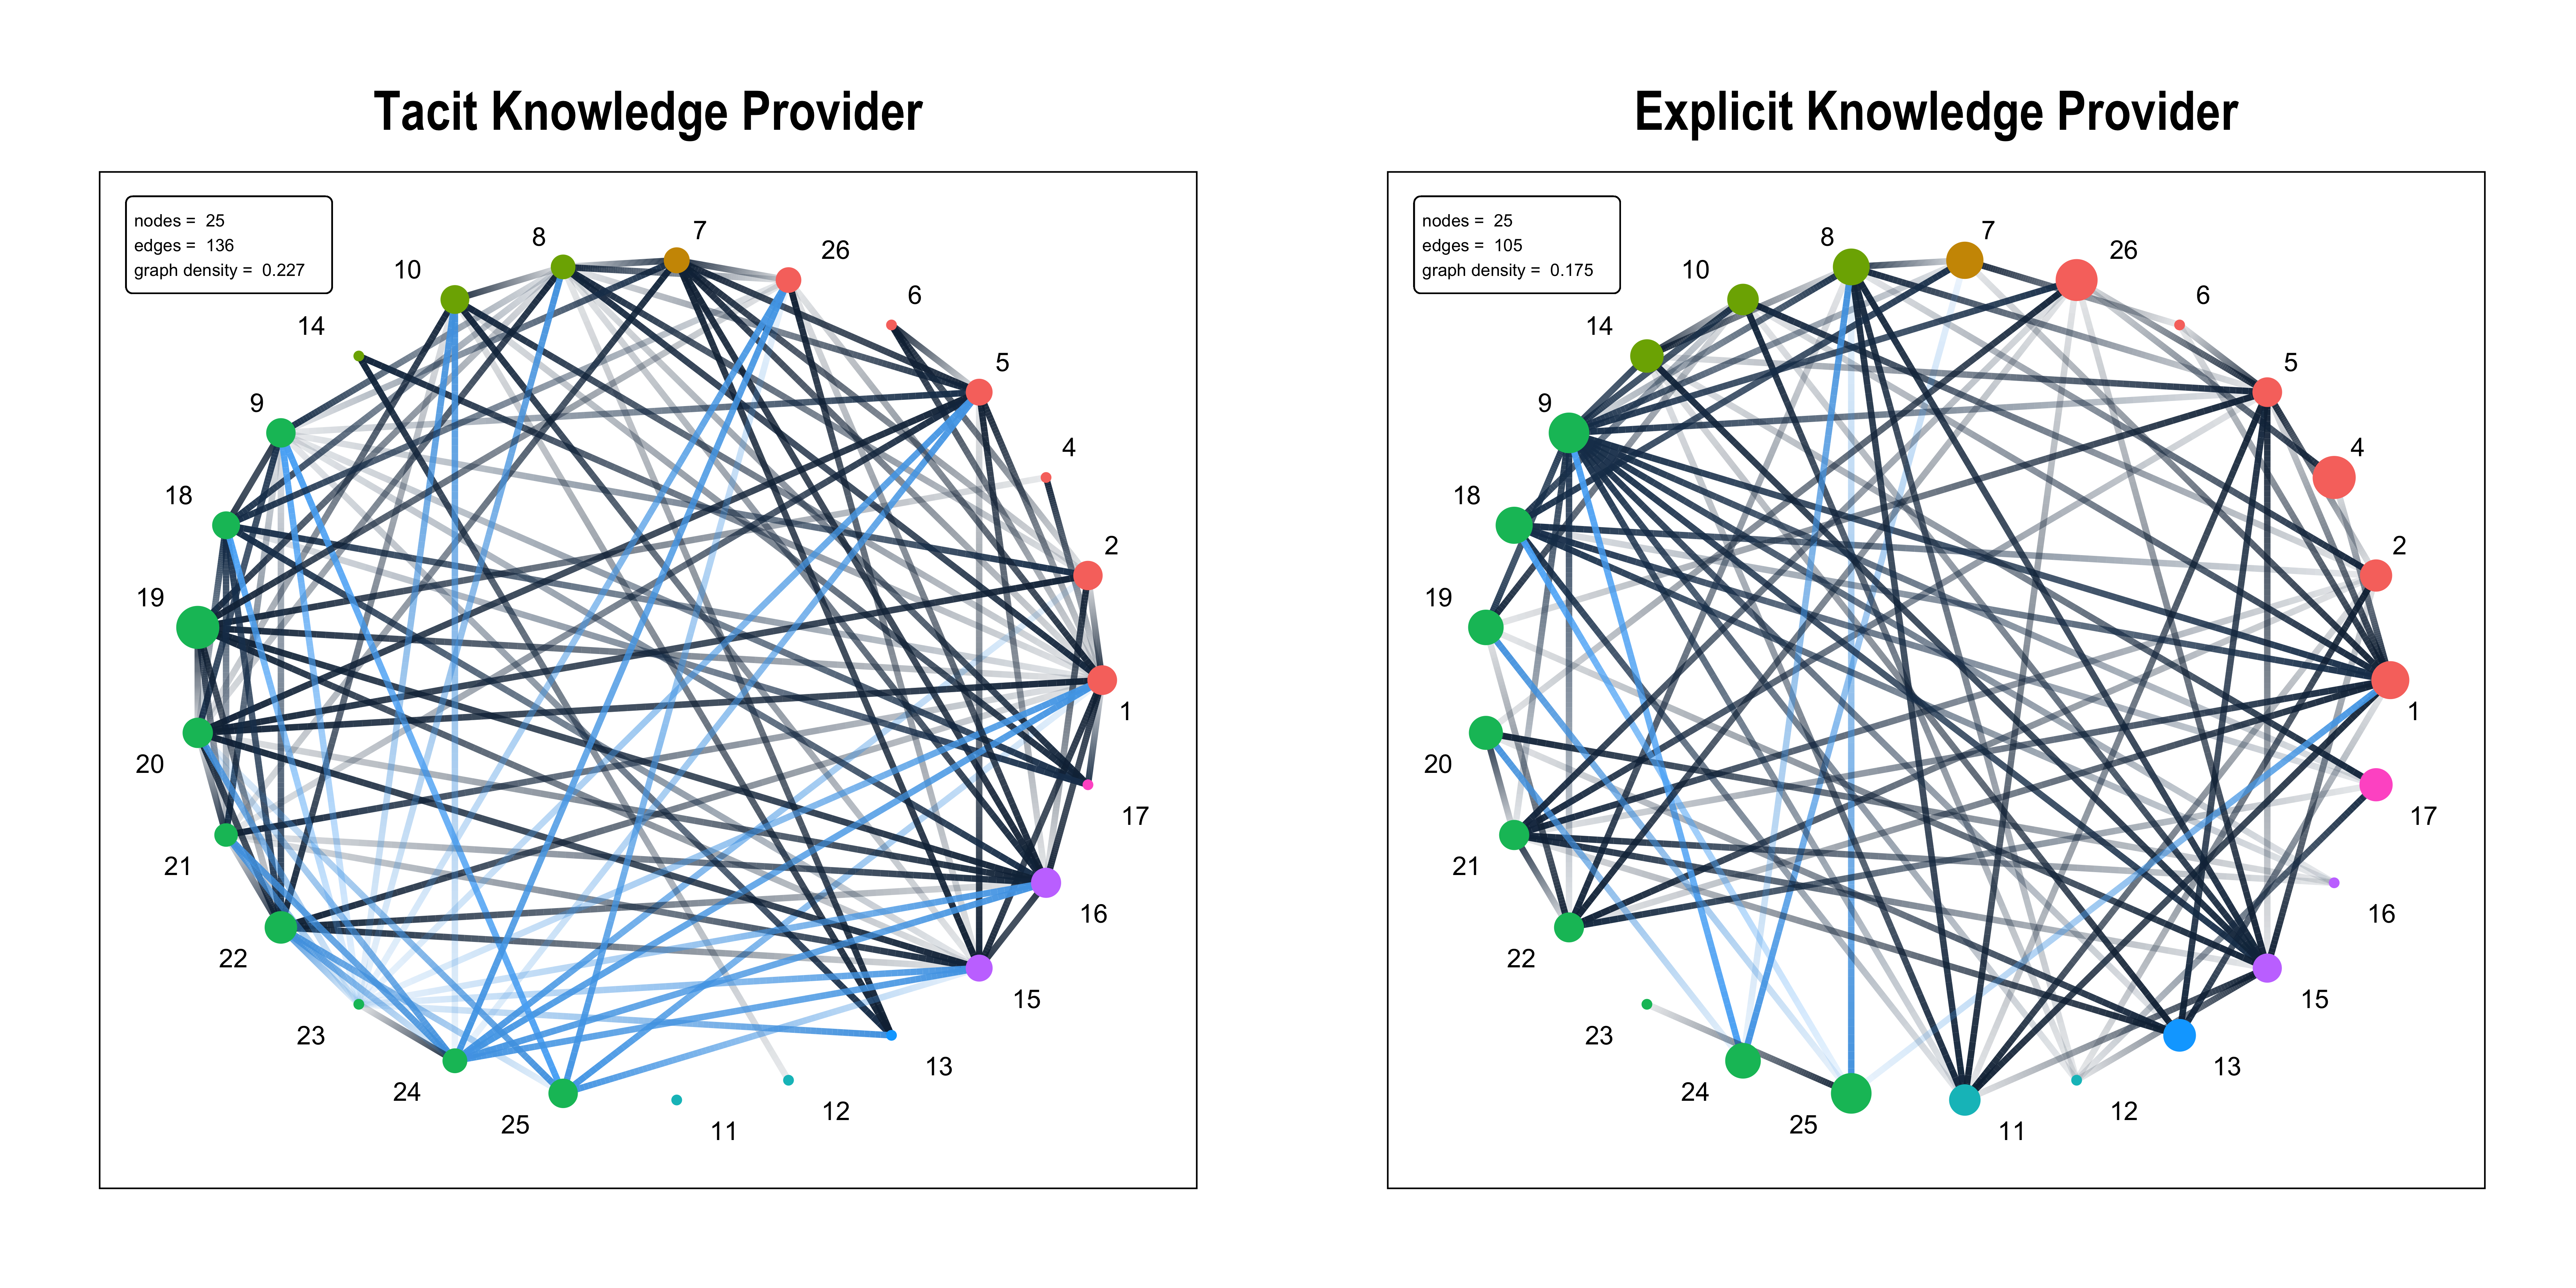
\includegraphics[width=1\linewidth]{Images/networks_case_2.png}
\caption[Knowledge networks for Case 2]{Knowledge networks for Case 2 (see text for an explanation of the different graphical representations).}
\label{fig:network_case_2} 
\end{sidewaysfigure}

\begin{sidewaysfigure}[hbt!]
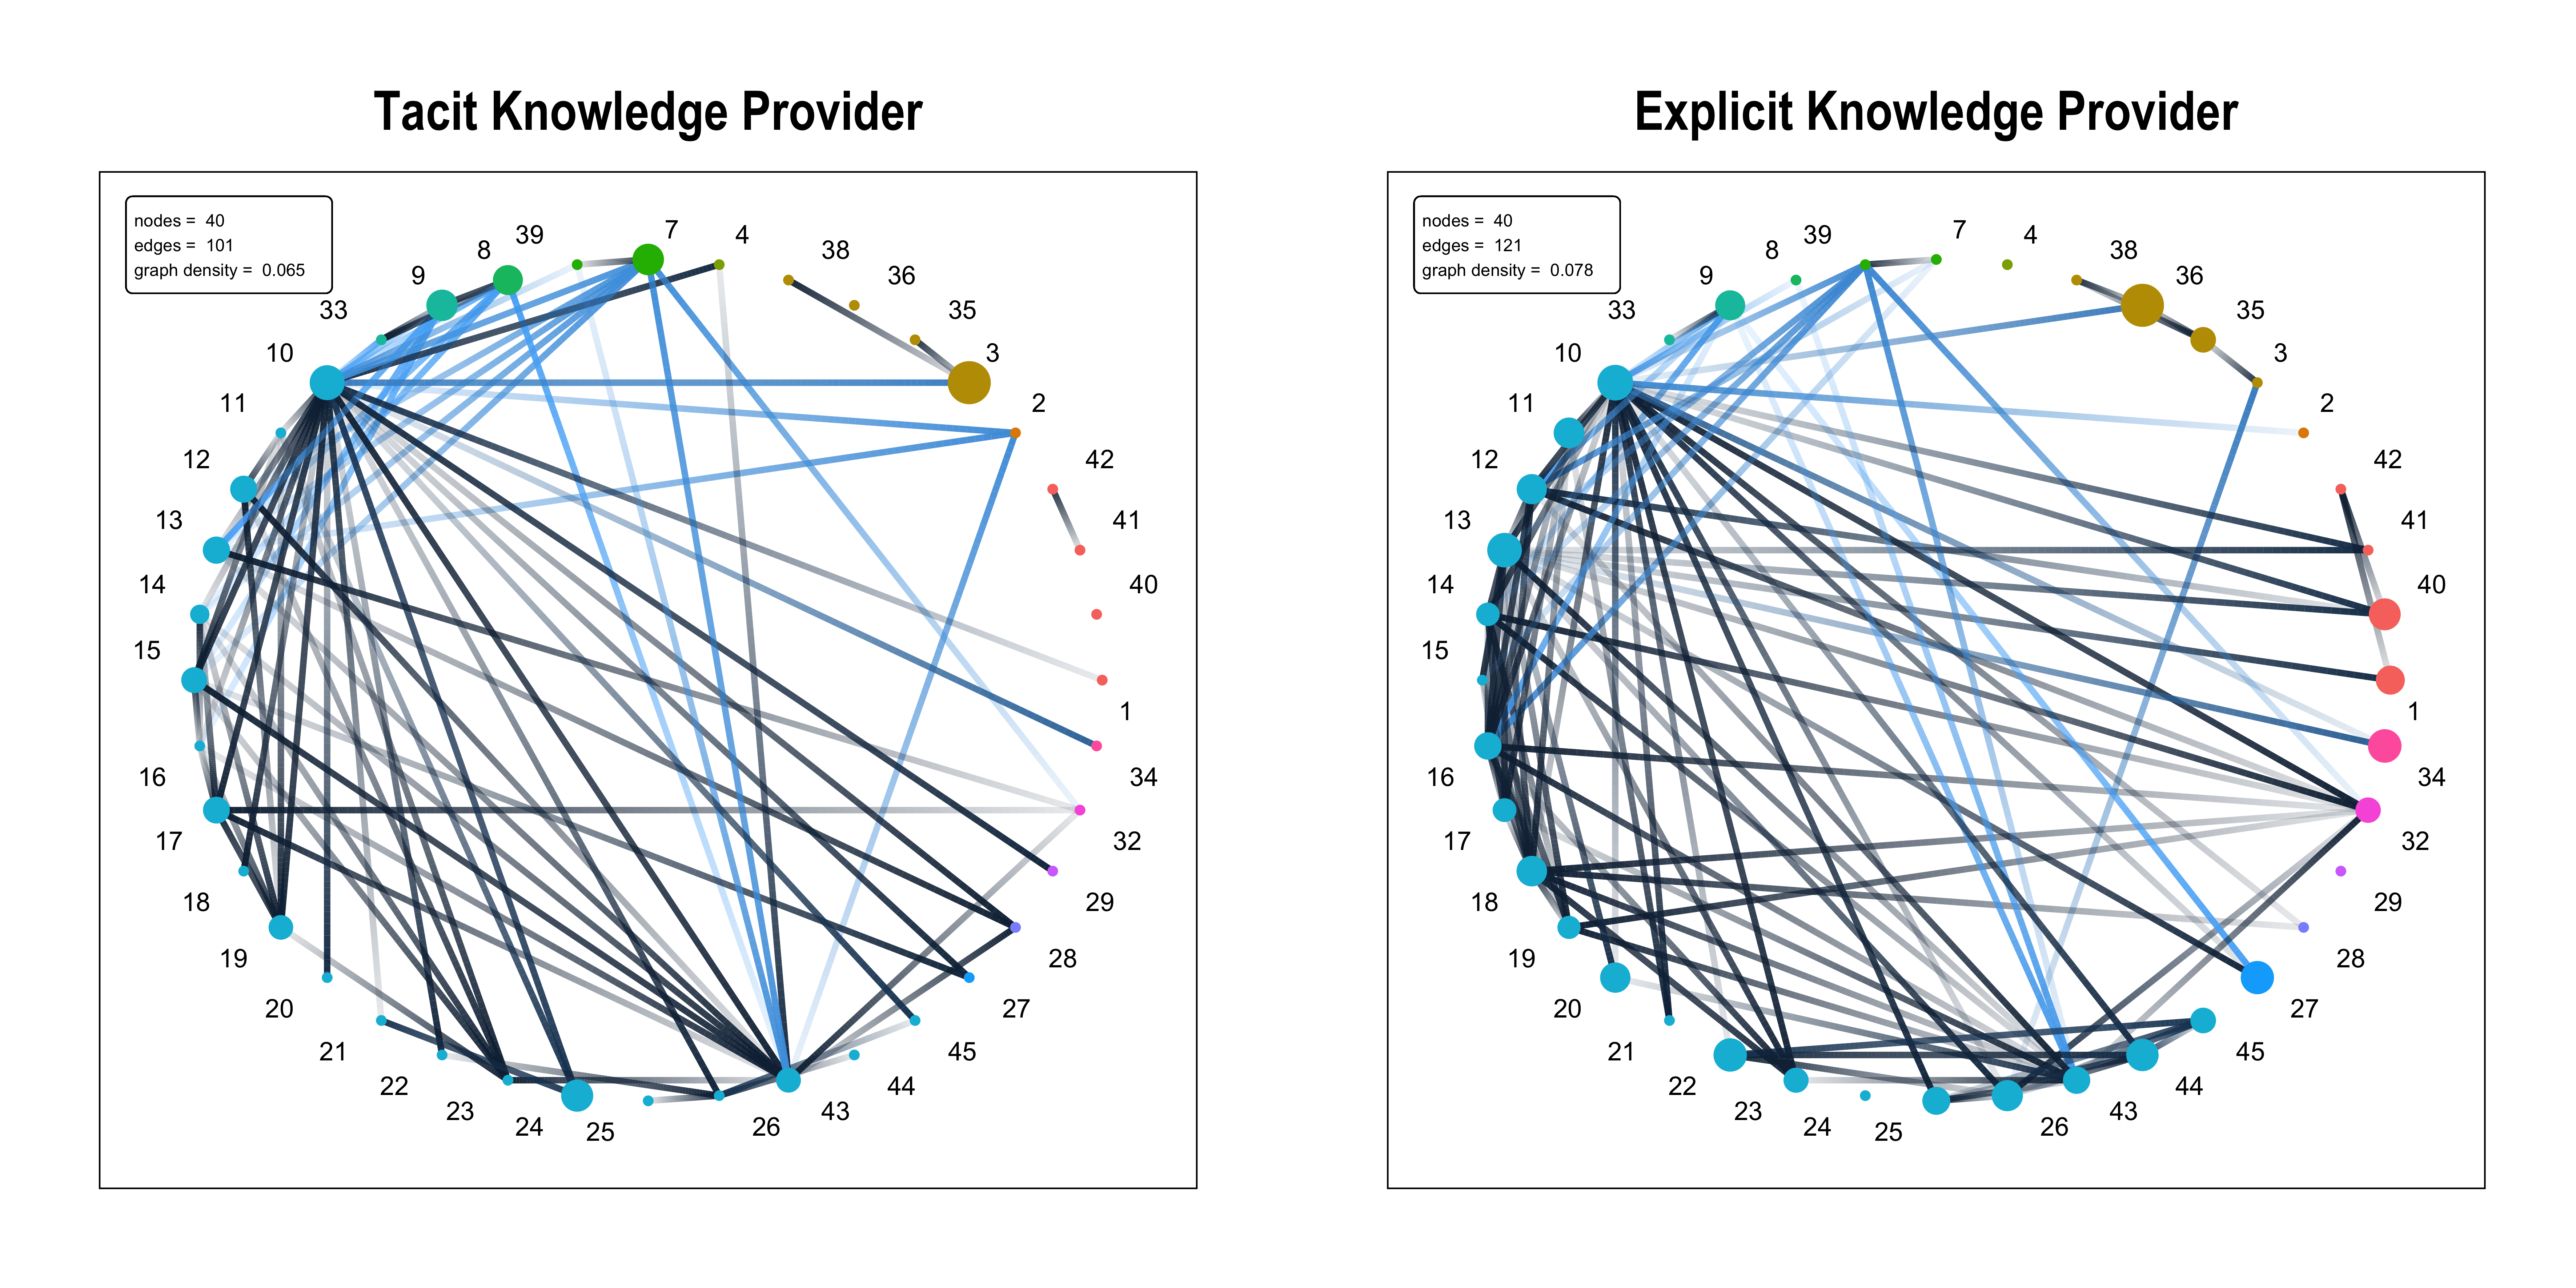
\includegraphics[width=1\linewidth]{Images/networks_case_3.png}
\caption[Knowledge networks for Case 3]{Knowledge networks for Case 3 (see text for an explanation of the different graphical representations).}. 
\label{fig:network_case_3} 
\end{sidewaysfigure}

\subsection{Broker roles}

Brokers are well placed to facilitate the flow of knowledge across organisational boundaries. By examining broker roles, one can assess knowledge diffusion in open innovation partnerships. Figure \ref{fig:gf_brokerage} presents a breakdown of \citeauthor{gould1989structures}'s \citeyearpar{gould1989structures} broker roles by knowledge type in each case (refer to Table \ref{tab:ergm_params} for an explanation of these roles).  \medskip

The mix of broker roles reveals something about knowledge sharing behaviour in each case. Looking at Case 1, the liaison broker role is dominant in the explicit knowledge provider network, indicating that participants are happy to pass on explicit knowledge from one partner to another partner. Some participants operate in a representative broker role, suggesting they are open to sharing their organisation's explicit knowledge with third-parties. The representative broker role is dominant in the tacit knowledge provider network, indicating that participants are open to sharing their organisational know-how and expertise with third-parties. As for Case 2, the liaison role dominates both the explicit and tacit knowledge provider networks. Participants in Case 2 appear willing to pass on all types of knowledge from one partner to another partner, a good sign of collaboration. The internal coordinator role dominates the explicit knowledge provider network in Case 3. Given that almost half the participants in Case 3 work for the same organisation, this is not surprising. The tacit knowledge provider network does not have a dominant broker role. Very few participants operate as itinerant brokers in any of the cases. Note that Figure \ref{fig:gf_brokerage} presents raw broker counts. The statistical significance of the different broker roles receives more attention in Chapter \ref{chp:ergm_result}. \medskip

\begin{figure}[hbt!]
\centering
\includegraphics[width = \linewidth]{Images/gf_brokerage.png}
\caption[Breakdown of broker roles]{Breakdown of \citet{gould1989structures} broker roles. Note $w_I$ = internal coordinator role, $b_O$ = liaison role, $b_{OI}$ = gatekeeper role, $b_{IO}$ = representative role, and $w_O$ = itinerant broker role.}
\label{fig:gf_brokerage}
\end{figure}

\section{Chapter summary}

Case 1 is an example of incremental inbound open innovation. Most of the knowledge exchanged in Case 1 is explicit. However, Case 1 was at an early stage when surveyed. Relationships vital for tacit knowledge exchange were still developing. One can categorise Case 2 as an example of coupled open innovation. Realising a farm system based on voluntary cow traffic is a radical innovation. Tacit knowledge features prominently in Case 2, even though many participants have to collaborate over great distances. This case was in its final stages and participants knew each other reasonably well, which may explain the relatively dense tacit knowledge provider network. Case 3 is an example of outbound open innovation. Using a combination of miniaturised electronic tags and cloud-based data analytics to coordinate honeybee research globally is considered radical innovation. As with Case 2, participants in Case 3 have to collaborate across vast distances. \medskip

The cases are very different in terms of open innovation archetype, the stage at which they are, demographic makeup, and brokerage patterns. One must be careful not to over-generalise the findings from each case. How the unique characteristics of each case shape tacit knowledge sharing will become more apparent in the following chapters. The next chapter (Chapter \ref{chp:ergm_result}) presents the results from the exponential graph modelling. It drills much deeper into the data presented in this chapter. The modelling results will highlight the statistical significance of exogenous factors influencing tacit knowledge sharing in the three open innovation partnerships. 